% Created 2023-04-17 Mon 23:25
% Intended LaTeX compiler: pdflatex
\documentclass[11pt]{article}
\usepackage[utf8]{inputenc}
\usepackage[T1]{fontenc}
\usepackage{graphicx}
\usepackage{longtable}
\usepackage{wrapfig}
\usepackage{rotating}
\usepackage[normalem]{ulem}
\usepackage{amsmath}
\usepackage{amssymb}
\usepackage{capt-of}
\usepackage{hyperref}
\usepackage{placeins}
\usepackage{gensymb}
\author{Christian Johnson}
\date{\today}
\title{CCN Notes}
\hypersetup{
 pdfauthor={Christian Johnson},
 pdftitle={CCN Notes},
 pdfkeywords={},
 pdfsubject={},
 pdfcreator={Emacs 28.2 (Org mode 9.6.3)}, 
 pdflang={English}}
\begin{document}

\maketitle
\tableofcontents




\section{Chapter 5 - Control Plane}
\label{sec:org54bc6a9}

\subsection{5.1 Introduction}
\label{sec:org86b6012}

In units 4.2 and 4.3 - Forwarding table and flow table (principal elements linking the Network layer and the control plane)
\begin{itemize}
\item These specify the local data-plane forwarding behavior for a router.
\end{itemize}

\subsubsection{Per Router Control}
\label{sec:org54326b7}
\begin{itemize}
\item the case where a routing algorithm runs in EVERY router (both a forwarding and routing function are contained in each router). Each router uses a \uline{routing component} - communicates with component in other routers. Computes forwarding table. \textbf{OSPF} and \textbf{BGP} protocols are based on this.
\end{itemize}

\begin{figure}[htbp]
\centering
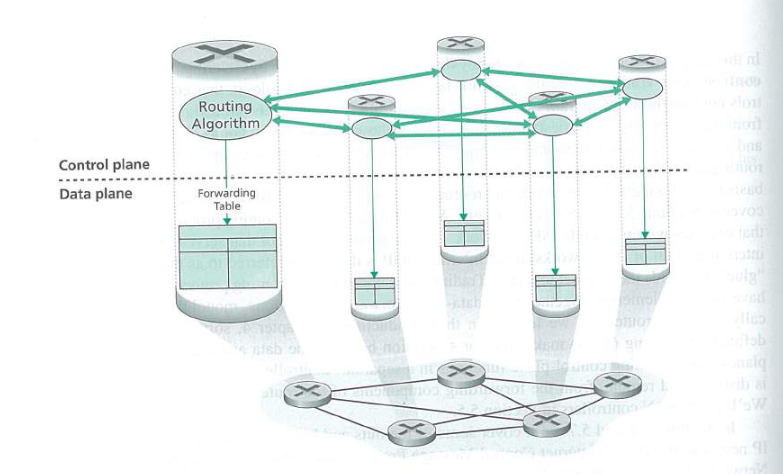
\includegraphics[width=.9\linewidth]{c:/Users/Christian/Documents/GitHub/Home/OrgFiles/Class Notes/Files/CCN Snippets/5.1.0.1.png}
\bicaption{Per-router control: Shows seperation between control and data plane}
\end{figure}

\subsubsection{Logically centralized control}
\label{sec:orgc38aff5}
\begin{itemize}
\item Controller distributes forwarding tables for each router.
\item Controller interacts with Control Agent (CA) via protocols to manage routers flow table. (CA's only job is communication).
\item Logically centralized control - routing control service is accessed at a single, central service point.
\end{itemize}

\begin{figure}[htbp]
\centering
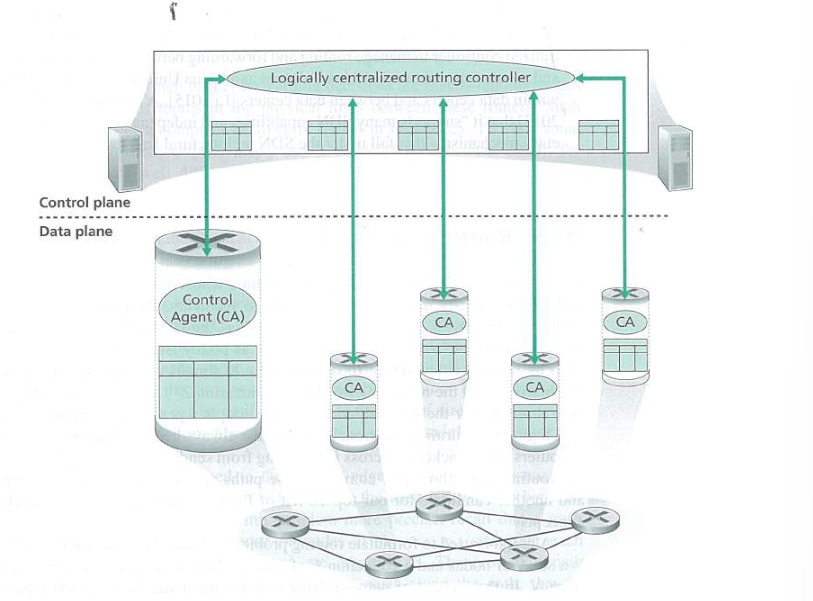
\includegraphics[width=.9\linewidth]{c:/Users/Christian/Documents/GitHub/Home/OrgFiles/Class Notes/Files/CCN Snippets/5.1.0.2.png}
\bicaption{Logically Centralized Control}
\end{figure}

\subsection{5.2 Routing Algorithms}
\label{sec:org00763fc}

Routing Algorithms - Determine the best path/route from senders to receivers.
---
\begin{center}
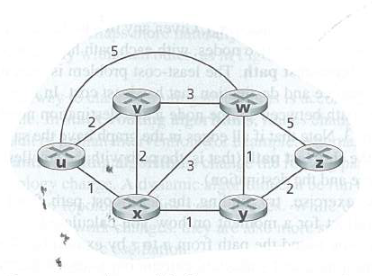
\includegraphics[width=.9\linewidth]{c:/Users/Christian/Documents/GitHub/Home/OrgFiles/Class Notes/Files/CCN Snippets/5.2.0.1.png}
\end{center}

---
Graphs are used to visualize routing.
\(G = (N,E)\)
\begin{itemize}
\item N = \# of Nodes
\item E = Collection of edges
\end{itemize}

Edge - a pair of nodes away from N.
Each node represents a router, edges connecting the nodes represent \emph{Physical Links} between each router.

Edges also have values - represent \emph{cost}.
\begin{itemize}
\item Edge cost corresponds to the physical length of the link (resistance/delay).
\end{itemize}
For an edge \((x,y)\), cost is \(c(x,y)\) as long as the edge is part of the network in question. If not, \(c(x,y)=\infty\).
We call \(x\) and \(y\) neighbours, if they are both in the same network.

Routing algorithms - goal is to \textbf{reduce cost}.
\begin{itemize}
\item a path - sequence of nodes \((x_{1}, x_{2}, ... , x_{p})\) where each pair \((x_{1}, x_{2}), (x_{2}, x_{3}), ... , (x_{p-1}, x_{p})\)
\end{itemize}
are edges in the network.
\begin{itemize}
\item Cost of a path - sum of all the edges along the path.

\textbf{Centralized Routing Algorithm}

\begin{itemize}
\item Computes least cost path between source and destination

\item Uses complete, global information about the network

\item Takes connection between all nodes/link costs as inputs

\item Algorithms with global information are known as \textbf{Link-state Algorithms}
\end{itemize}
\end{itemize}


\textbf{Decentralized Routing Algorithm}

\begin{itemize}
\item Calculation (for least cost path) carried out in iterative, distributed manner
\item No one node has complete information about the cost of all links, knows only about connected/directly attatched links.
\end{itemize}


Static VS. Dynamic Routing Algorithms:
Static routes change slowly over time (usually manually)
Dynamic routes change routing paths as traffic or network topology changes.
\begin{itemize}
\item Dynamic is more responsive, but more susceptible to issues.
\end{itemize}


Load Sensitive VS. Load Insensitive:
Load sensitive link costs change dynamically to reflect current congestion.
Insensitive links do not reflect their current conditions.

\subsubsection{5.2.1 Link State (LS) Routing Algorithms}
\label{sec:org178b995}

All link costs are known in a link state - each node broadcasts link-state packets to ALL other nodes in network.

Packet: Identities and costs of the attached links.

\textbf{Link State Broadcast Algorithm}

\begin{enumerate}
\item Djikstra's Algorithm
\label{sec:org97632e8}

\begin{itemize}
\item link state routing algorithm.
\item Iterative
\item After the kth iteration, least cost paths are known to k destination nodes.
\item These k paths have among them the k smallest costs
\end{itemize}


\textbf{Terminology}
\begin{itemize}
\item \(D(v)\): Cost of the least cost path from source to destination \emph{v}
\item \(p(v)\): Previous node (neighbours with \emph{v}) along the current least-cost path
\item \(N'\): subset of nodes; v is inside \(N'\) if the least-cost path is definitely known.
\end{itemize}


\clearpage

\begin{figure}[htbp]
\centering
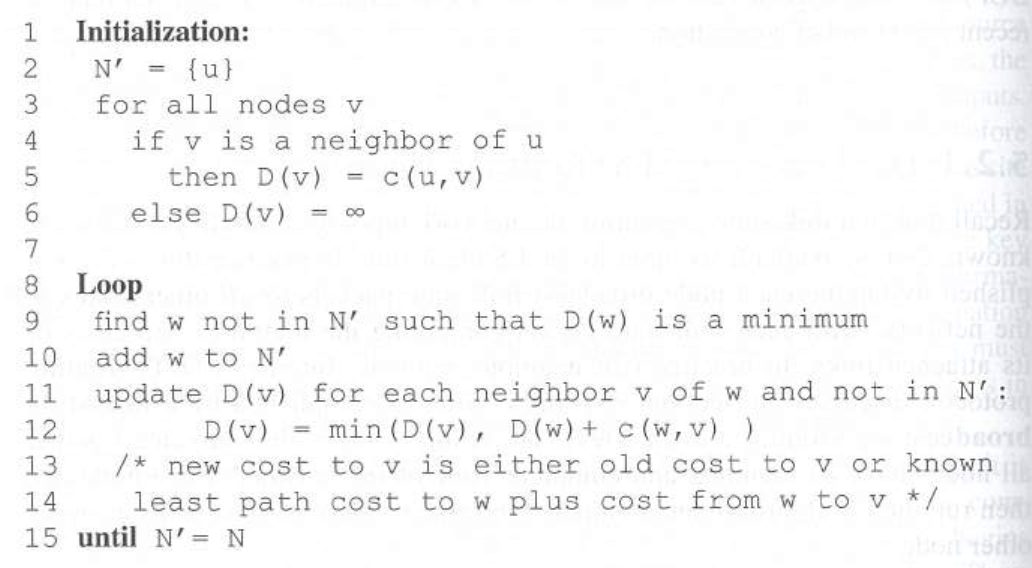
\includegraphics[width=.9\linewidth]{c:/Users/Christian/Documents/GitHub/home/OrgFiles/Class Notes/Files/CCN Snippets/5.2.1.1.png}
\bicaption{Link-State Algorithm for Source "u"}
\end{figure}

\begin{figure}[htbp]
\centering
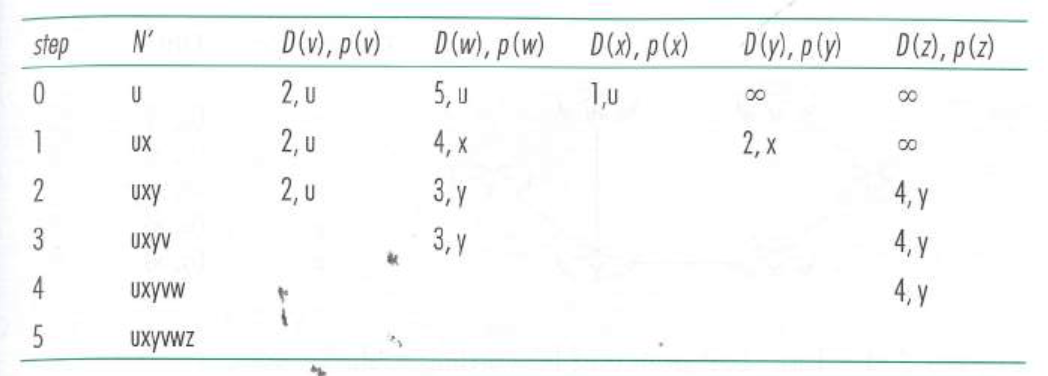
\includegraphics[width=.9\linewidth]{c:/Users/Christian/Documents/GitHub/home/OrgFiles/Class Notes/Files/CCN Snippets/5.2.1.2.png}
\bicaption{Link-State Algorithm for above "Graph of a Network"}
\end{figure}

\begin{figure}[htbp]
\centering
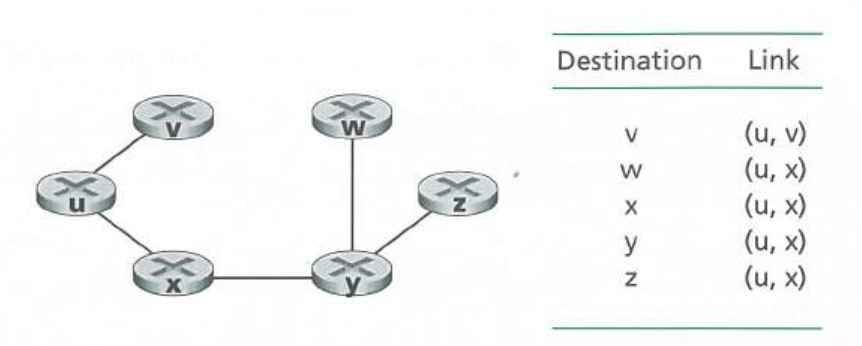
\includegraphics[width=.9\linewidth]{c:/Users/Christian/Documents/GitHub/home/OrgFiles/Class Notes/Files/CCN Snippets/5.2.1.3.png}
\bicaption{Resultant Least-Cost Path and Routing Table}
\end{figure}

\clearpage

Potential Issues:
With circular routing paths, the algorithm can detect an oscillating pattern on each new transmission, resulting in repeating route changes. Possible solution: ensure that not all routers are running the same LS algorithm at the same time.

Self Synchronization: can occur no matter when or in what phase a router starts its algorithm. Can be avoided by randomizing the time a router sends a link advertisement.
\end{enumerate}

\subsubsection{5.2.2 Distance-Vector (DV) Routing Algorithm}
\label{sec:org257f67f}

\begin{itemize}
\item Iterative - distribution continues until no more information is exchanged
\begin{itemize}
\item Asynchronous - Does not require nodes to operate in sync.
\end{itemize}
\item Distributed - each node receives information from one or more \emph{directly attached} neighbors, performs a calculation, then re-distributes the results.
\end{itemize}


Bellman-Ford Equation: \(d_{x}y = min_{v}[c(x,v)+d_{v}(y)]\)
\begin{itemize}
\item \(min_v\) - includes all of x's neighbors
\item This equation is what provides the entries to node x's forwarding table
\end{itemize}

\begin{figure}[htbp]
\centering
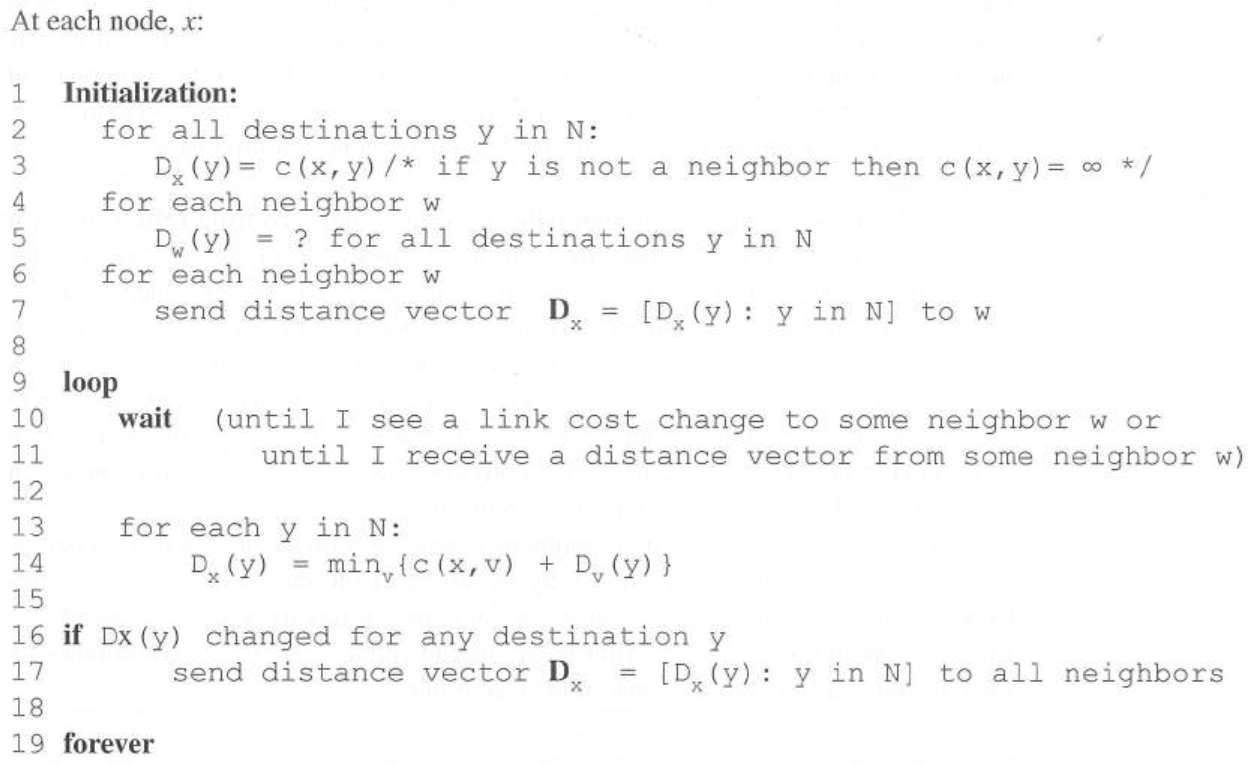
\includegraphics[width=.9\linewidth]{c:/Users/Christian/Documents/GitHub/home/OrgFiles/Class Notes/Files/CCN Snippets/5.2.2.1.png}
\bicaption{Distance Vector (DV) Algorithm}
\end{figure}

Nodes update their distance-vector estimate either when they see a cost change in one of the directly attached links, or it receives a distance-vector update from a neighbor.

Where the LS algorithm is centralized, and requires each node to maintain a complete map of the entire network, the DV algorithm focuses on computing the neighbouring node that is the next-hop router along a route to the destination (uses costs for each neighbour instead of entire network).

DV algorithms avoid what is known as a \textbf{Routing Loop} (or an infinite cycle caused by incomplete information) with a \emph{Poisoned Reverse}.

\subsubsection{DV vs LS}
\label{sec:orged3ba5c}

DV talks \uline{only} to its connected neighbours
LS talks to the \uline{entire} network

\begin{itemize}
\item Message Complexity - LS is more complex, since it requires more information to be sent and stored. Also means that any changing information must be sent to the entire network.
\item Speed of Convergence - DV algorithm is slower (requires more processing, since each node has less information). Also susceptible to routing loops and count to infinity errors.
\item Robustness - LS provides a degree of seperation, since each router conducts its own calculations. LS nodes can also only provide incorrect information for one of its attached links, where DV has no such limitation.
\end{itemize}

\subsection{5.3 Intra-AS Routing in the Internet: OSPF}
\label{sec:org821d227}

Need to adapt our view of the internet.
Can't simply view it as a collection of arbitrary routers

\begin{itemize}
\item Scale - Given how many routers we have as part of the internet, it would require a prohibitive amount of storage to generate routing tables and algorithms for the entire network.
\item Administrative Autonomy - Internet is a collection of ISP's. Each ISP is independently operated and maintained.
\end{itemize}


These issues can be resolved by organizing routers into \textbf{Autonomous Systems} or AS's.
Each AS consists of a groups of routers under the same administrative control.
They are identified with their Autonomous System Number (ASN).
Routers within the same AS all use the same routing algorithm and have information about each other. The routing algorithm running in an autonomous system is called an \textbf{intra-autonomous system routing protocol}.

\subsubsection{Open Shortest Path First (OSPF)}
\label{sec:orga4db1c8}

OSPF and the related IS-IS are used for intra-AS routing.
OSPF - link state protocol. Uses flooding of link state information and a Djikstra least-cost path algorithm.

Each router constructs a complete topological map (graph) of the entire AS. Each router runs Djikstra's shortest path algorithm to determine a shortest-path tree to all subnets. Individual link costs are configured by the network admin. OSPF broadcasts to \emph{all} other routers in the network.

OSPF Features:
\begin{itemize}
\item Security - OSPF exchanges can be authenticated. Prevents untrusted routers from participating. 2 possible types of authentication: simple, and MD5. (Simple - same password on each router, password included in the packet in plaintext) (MD5 - Based on shared, secret keys that are configured in every router. Each packets content is computed into an MD5 hash, then includes the hash value in the packet. receiving packet decodes the hash with the shared key. Sequence numbers also used.)
\item Multiple same-cost paths - OSPF allows multiple paths to be used if they a share the same cost to a destination.
\item Integrated support (unicasting and multicast routing) - Multicast OSPF (MOSPF) - simple extensions to OSPF. Use sexisting OSPF database, adds new type of link state advertisement to existing OSPF link-state broadcast mechanism.
\item Support for hierarchy within a single AS - OSPF AS can be configured into hierarchical "areas". Each area runs on its own OSPF Link state routing algorithm. Each area also has one/more border routers responsible for routing packets outside the area. Exactly ONE OSPF area is configured as the backbone (primary purpose to route packets throughout the AS.)
\end{itemize}

\subsection{5.4 Routing Among the ISPs: BGP}
\label{sec:orgd0b40ec}
OSPF is responsible for routing across multiple areas within the same AS.
When we need to route across multiple AS's however, we use an \textbf{Inter-Autonomous System Routing Protocol}.
Requires the connected AS's to run the same inter autonomous system routing protocol.
Most common one known as the \textbf{Border-Gateway Protocol} or BGP.

\subsubsection{5.4.1 Role of BGP}
\label{sec:org64c27cc}
In BGP, packets aren't routed to specific destination addresses, but to CIDRized prefixes (represent a subnet or collection of subnets).

BGP provides each router a way to:
\begin{itemize}
\item Obtain prefix reachability information from neighboring AS's - Allows each subnet to advertise its existance to the rest of the internet.
\item Determine the "best" routes to the prefixes
\end{itemize}

\subsubsection{5.4.2 Advertising BGP Route Information}
\label{sec:orgd7f776c}
In every AS, each router is either a \textbf{Gateway Router} or an \textbf{Internal Router}.
Gateway routers are on the edge of the AS and connect directly to routers in other AS's.
Internal routers connect only to routers in their own AS. 

\subsubsection{5.4.3 Determining the best routes}
\label{sec:orgfab9cc0}
When a router advertises a prefix across a BGP connection, it includes alongside the prefix sever \textbf{BGP Attributes}. Prefixes and attributes together are called a route.
Two important attributes: AS-PATH and NEXT-HOP.
AS-PATH: List of the AS's the advertisement has passed through.
NEXT-HOP: The IP address of the router interface that began the AS-PATH. 

\begin{enumerate}
\item Hot Potato Routing
\label{sec:orgcb65d89}
In hot potato routing, the route chosen is the one with the least cost to the NEXT-HOP router. Consults the routing table for the intra-AS information. Determines the lowest cost path to the destination based on the lowest cost from each progressive router. 

\item Route Selection Algorithm
\label{sec:org0dc021c}
For any given prefix, the input into the route selection algorithm is the set of all routes to that prefix that have been learned and accepted by the router. If there's more than one route the algorithm uses the following rules to pare down the selections until one remains.

\begin{enumerate}
\item Route is assigned a \emph{local preference} value. Could be set by router, or learned from another router in the same AS. Routes with the highest local preference are selected.
\item From the remaining routes (all have the same highest local pref. value) the route with the shortest AS-PATH is selected.
\item From remaining (all with highest local pref. value and same AS-PATH length) hot potato routing is used to find the route with the closest NEXT-HOP router.
\item If more than one route remains, the router uses BGP identifiers to select the route.
\end{enumerate}
\end{enumerate}

\subsubsection{5.4.4 IP-Anycast}
\label{sec:org33ebf22}
BGP is also used to implement the IP-Anycast Service, commonly used in DNS.
We sometimes want to replicate information on servers other than the origin of that information. 
We can use BGP to advertise Servers that are configured with the same IP address using IP Anycast.

This service is also used by DNS to direct DNS queries to the closest root DNS Server. 

\subsubsection{5.4.5 Routing Policy}
\label{sec:org31fcb29}
AS routing policy can trump all other considerations when a router selects a route. 

\subsubsection{5.4.6 Putting the Pieces together: Obtaining Internet Presence}
\label{sec:org9307aad}
Internet connectivity is the first step in establishing a presence online.
Must connect to a local ISP.
Local Gateway Router will be connected to a router in your ISP.
ISP provides you with an IP range (CIDR format, /24 eg).
Once you have your gateway and IP range, you assign an IP address from that range to each service you want to connect (Web server, Mail server, DNS Server, Gateway Router, and other servers and netwroking devices).
Also need to connect with an Internet Registrar to get a domain name and connect to the DNS system.
In order to make this domain and the hosts on it available to the outside internet, you must provide a way to route from the internet at large through your servers.
This is accomplished with BGP. Your local ISP will use BSP to advertise your prefix so that its able to forward datagrams to the proper destinations within your AS.

\subsection{5.5 The SDN Control Plane}
\label{sec:orgf71bbf3}

SDN Control Plane - network wide logic that controls packet forwarding among a network's SDN-enabled devices.

Four Key Characteristics of an SDN Architecture:
\begin{itemize}
\item Flow based forwarding - packet forwarding by SDN-controlled switches, based on any number of header field values. OpenFlow1.0 abstraction allows 11 different header values.
\item Seperation of Data Plane and Control Plane - data plane consists of network's switches, control plane consists of servers and software that determine/manage the switches flow tables.
\item Network control functions: external to data-plane switches: SDN control plane is implemented in software. This software executes on servers that are \emph{distinct} and \emph{remote} from the networks switches. Control plane consists of two pieces: SDN controller (network operating system) and a set of network control applications. Controller - accurate state information, provides to network control application and provides the means through which these appliations can monitor/program/control the underlying network devices.
\item Programmable Network - Network is programmable through the network applications running in the control plane. Applications represent the \textbf{Brains} of the SDN control plane. Use API's provided by the SDN to specify and control the data plane in the network devices.
\end{itemize}


SDN \emph{unbundles} the existing network functionality. Previously, it was all contained in a single provider, now data plane switches, SDN controllers, and network control applications can all be provided by seperate vendors. 

\subsubsection{5.5.2 SDN Control Plane: SDN Controller and SDN Network-Control Applications}
\label{sec:org3ecbba6}

SDN Control Plane divides into two sections:
SDN controller and SDN network-control applications.

Controllers functionality:
\begin{itemize}
\item \emph{Communication Layer: communicating between the SDN controller and controlled network devices.} Protocol needed to transfer information between controller and device. This protocol is the lowest later of the controller architecture.
\item \emph{Network wide state management layer.} The ultimate control decisions made by the SDN control plane requires that the controller hace up-to-date information about the state of the networks hosts, links, switches, and other SDN controled devices. Switch's flow table contains counters - useful to applications. Since ultimate aim of the control plane is to determine flow tables for the various controlled devices, controller may maintain copies of these switch's tables.
\item \emph{Interface to the network-control layer.} Controller interacts with network-control applications through "northbound" interface. This API allows network-control applications to read/write network state and flow tables within the state-management layer.
\end{itemize}
\begin{center}
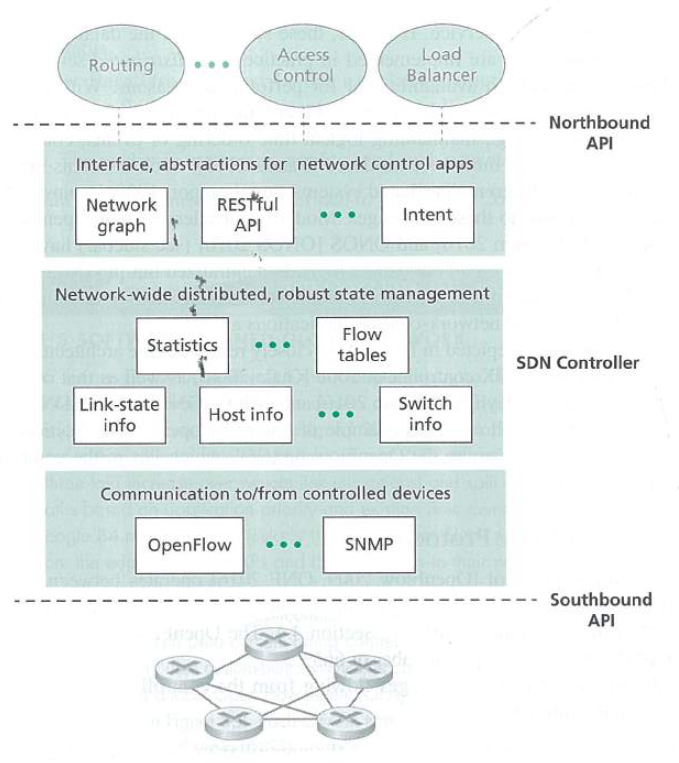
\includegraphics[width=.9\linewidth]{c:/Users/Christian/Documents/GitHub/home/OrgFiles/Class Notes/Files/CCN Snippets/5.5.0.1.png}
\end{center}

SDN Controller typically considered centralized. Services and databases used to hold state information are implemented with distributed servers (allows for fault tolerance, high availability, or performance). 

\subsubsection{5.5.2 Open Flow Protocol}
\label{sec:orgee756cb}

OpenFlow Protocol operates between an SDN controller and an SDN controlled switch or other device implementing OpenFlow API. Operates over TCP, default port number of 6653.

Important Messages flowing from Controller to Controlled Switch:
\begin{itemize}
\item \emph{Configuration.} Allows controller to query and set a switch's configuration
\item \emph{Modify-State.} Used by Controller to add/delete/modify entries in the Switch's flow table, and set switch port properties.
\item \emph{Read-State.} Used by Controller to collect statistics and counter values from switch's flow table and ports.
\item \emph{Send-Packet.} Used by Controller to send specific packer out of a specific port at the controlled switch.

Messages flowing from Switch to the Controller:
\begin{itemize}
\item \emph{Flow-removed.} Informs Controller that a flow table entry has been removed. (eg by timeout, or result of \emph{modify-state} message)
\item \emph{Port-Status.} Used by switch to inform controller of a change in port status.
\item \emph{Packet-In.} Packet arriving at a switch port and not matching a flow table entry is sent to controller for additional processing. Matched Packets may also be sent to controller. \emph{Packet-in} message used to do this.
\end{itemize}
\end{itemize}

\subsubsection{5.5.3 Data and Control Plane Interaction}
\label{sec:org74356fd}

\begin{figure}[htbp]
\centering
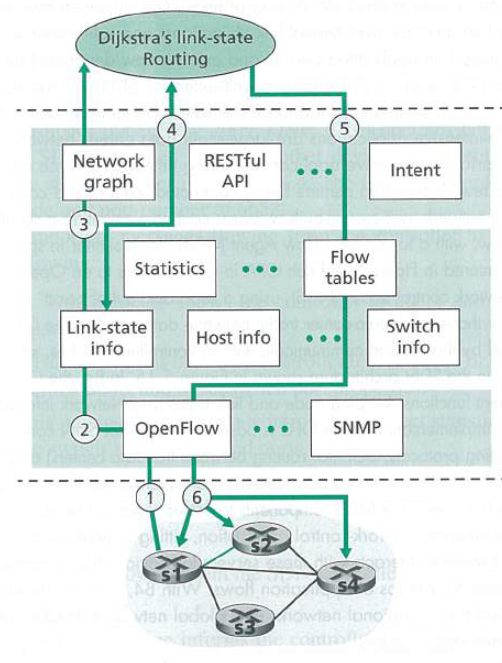
\includegraphics[width=.9\linewidth]{c:/Users/Christian/Documents/GitHub/home/OrgFiles/Class Notes/Files/CCN Snippets/5.5.3.1.png}
\bicaption{Data and Control Plane Interaction: Example}
\end{figure}

This diagram illustrates an example in which Djikstra's algorithm is used to find path routes.
Djikstra's algorithm is executed as a seperate application, outside the packet switches.
Packet switches send link updates to the SDN controller, not each other.

\begin{enumerate}
\item Switch S1 experiences link failure between self and S2. Notifies SDN controller of link-state change using OpenFlow \emph{port-status} message
\item SDN controller receives, notifies link-state manager which updates link-state database
\item Network-control application that implements Djikstra's link-state routing is previouslt registered to be notified when link-state changes. That appliaction receives notification of change.
\item Link-state routing application interacts with link-state manager to get updated link-state - may also consult other components in the state-management layer. Computes least-cost paths.
\item Link-state routing application interacts with the flow table manager, determines flow tables to be updated.
\item Flow table manager uses OpenFlow protocol to update flow table entries at affected switches.

(s1 - now routes to s2 via s4; s2 - now receives packets from s1 via s4; s4 - now routes packets from s1 to s2)
\end{enumerate}

\subsection{5.6 ICMP: The internet Control Messaging Protocol}
\label{sec:org12c5f19}
ICMP is used by hosts and routers to communicate network-layer information to each other. Most typical use is for error reporting.

\begin{itemize}
\item Often considered part of IP, but architecturally it lies above IP. ICMP
\item Messages carried inside IP datagrams, as IP payload.
\item ICMP messages have type and code fields. Contains the header and first 8 bytes of the IP datagram that caused the ICMP message to be generated (in the case of an error message, it would be the IP datagram with an error).
\item Ping works by sending an ICMP type 8 code 0 to the specified host. Destination host sees this, and responds with a type 0 code 0.
\end{itemize}
\begin{center}
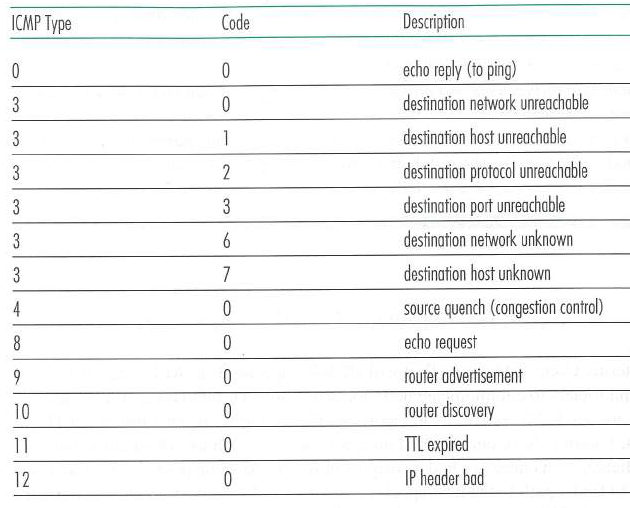
\includegraphics[width=.9\linewidth]{c:/Users/Christian/Documents/GitHub/home/OrgFiles/Class Notes/Files/CCN Snippets/5.6.0.1.png}
\end{center}

Traceroute is also implemented using ICMP. Sends a series of ordinary IP datagrams to the destination, each with a UDP segment with an unlikely 18 UDP port number. They have sequentially increasing TTL's. The source starts timers for each datagram. Once the nth datagram arrives at the nth router, that router sees that the TTL has expired, discards the packet, and sends an ICMP warning (type 11 code 0) to the source. When the ICMP arrives, it tells the source router the round-trip time, name, and IP address of the nth router.

\subsection{5.7 Network Management and SNMP}
\label{sec:orge3c3358}
Network Management includes the deployment, integration,
and coordination of the hardware, software, and human elements to monitor, test, poll, configure, analyze, evaluate, and control the network and element resources to meet the real-time, operational performance and Quality of Service requirements at a reasonable cost.

\section{Chapter 6 - Link Layer and LAN}
\label{sec:org6f7e3ed}

\subsection{6.1 Introduction to Link Layer}
\label{sec:org36ff5f0}

Node - any process that runs a link-layer protocol.
Links - Communication channels that connect adjacent nodes along the communication path.
Over a given link → transmitting node encapsulates the datagram in a \textbf{link-layer frame} and transmits that frame to the link.

\subsubsection{6.1.1 Services Provided by the Link Layer}
\label{sec:orgcfb4155}

\begin{itemize}
\item Framing - almost all link-layer protocols \emph{encapsulate} each network layer datagram in a link-layer \emph{frame} before transmission. Frame consists of a \uline{data field}, where the datagram is inserted, and several \uline{header fields}. Structure specified by link-layer protocol.
\item Link access - Medium Access Protocol (MAC) specifies rules under which a frame is transmitted to a link. For simple routes with few linkages, MAC protocol is simple or nonexistant (sener can send whenever the link is idle). More complicated - multiple nodes share a single broadcast link. MAC address works to coorfinate between nodes.
\item Reliable Delivery - guaruntees to move each network layer datagram across a link without error. Can be achieved with acknowledgements and retransmission. Used for links that are prone to high error rates (wireless links eg) to correct errors locally instead of forcing an end to end retransmission. Unneccessary for low error links.
\item Error Detection and Correction - Link-layer hardware in receiving node can incorrectly decide that bit is zero when it was actually one and vice verse. Error is produced by signal attenuation and electromagnetic noise. Many protocols provide methos to find these errors and prevent them sending. (Error detection bits in frames and receivers perform error check.)
\end{itemize}

\subsubsection{6.1.2 Where is the Link-Layer Implemented?}
\label{sec:orga73d5e4}

Link layer mostly implemented in the \textbf{network adapter} aka \textbf{Network Interface Card} (NIC). Heart of the NIC - link layer controller. Single chip designed to implement link layer services. (Link layer mostly implemented in hardware).
\begin{figure*}
\centering
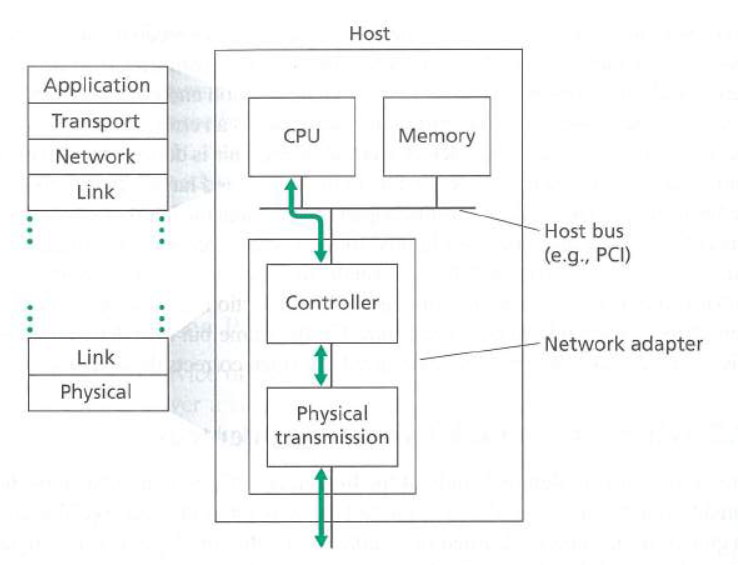
\includegraphics[width=.9\linewidth]{c:/Users/Christian/Documents/GitHub/Home/OrgFiles/Class Notes/Files/CCN Snippets/6.1.2.1.png}
\bicaption{Typical Host Architecture (Network Adapter)}
\end{figure*}

Sending Side - controller takes datagram (already been created and stored in host memory) encapsulates it in a link-layer frame, then transmits the frame to the communication link. Receiving side - controller receivess entire frame, extracts layer datagram. If link layer performs error detection, then sending controller sets error bits in the datagram and receiving controller that performs error check.

\subsection{6.2 Error Detection and Correction Techniques}
\label{sec:org14c04ce}
\begin{figure*}
\centering
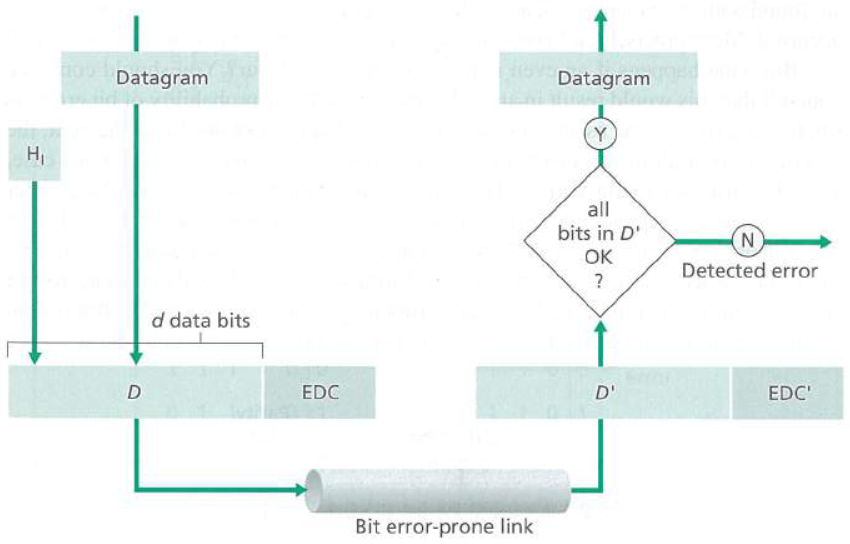
\includegraphics[width=.9\linewidth]{c:/Users/Christian/Documents/GitHub/Home/OrgFiles/Class Notes/Files/CCN Snippets/6.2.0.1.png}
\bicaption{Detection and Correction Scenario}
\end{figure*}

At sending node, data (D) is to be corrected and protected against bit errors. It is augmented with error detection and correction bits (EDC).
Typically, protected information includes datagram, link-level addressing information, sequence numbers, and other fields in the link frame header.
D and EDC are sent to the receiving node in a link level frame. At the receiving node, D' and EDC' are received (sequences of bits) D and EDC may differ form D' and EDC' (in-transit bit flips). Use error detection techniques to determine whether D'=D (The receiver only has D' and EDC' to work with). These techniques aren't perfect, may still be undetected errors. 

\subsubsection{6.2.1 Parity Checks}
\label{sec:orgb218015}
\begin{figure*}
\centering
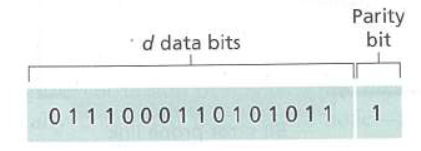
\includegraphics[width=.9\linewidth]{c:/Users/Christian/Documents/GitHub/Home/OrgFiles/Class Notes/Files/CCN Snippets/6.2.1.1.png}
\bicaption{Parity Bits Example}
\end{figure*}
Uses a single \textbf{Parity Bit}.
If D had \emph{d} bits, then the sender includes one additional bit. Chooses that bit's calue such that the total number of 1's is even.
If there are already an even number of 1's before the parity bit is introduced, then the parity bit would be 0 and would result in undetected errors.
Errors typically occur in "bursts". Makes single bit parity relatively imprecise - need a better method.
We can use two dimensional parity to allow us to correct individual errors more easily.
The receivers ability to both detect and correct is called \textbf{Forward Error Correction} (FEC). This can potentially reduce the number of sender retransmissions, and allows for immediate error correction at the receiver (eliminates Round Trip Delay from waiting on ACKS/NACKS).
\begin{figure*}
\centering
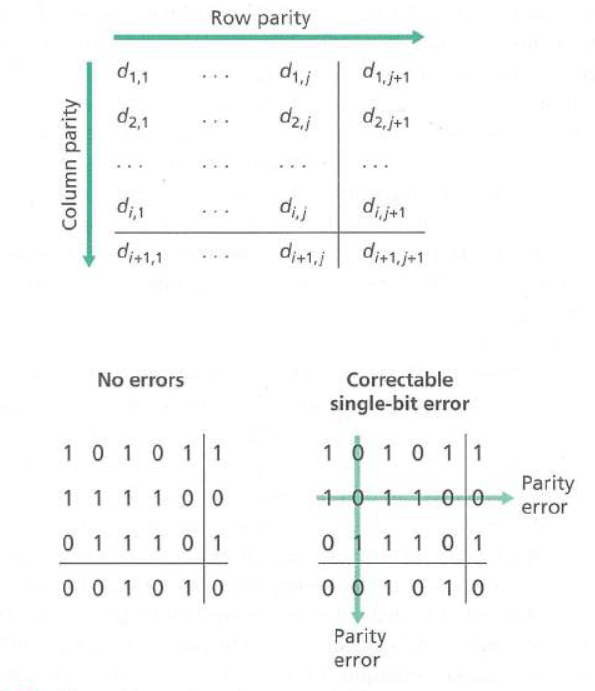
\includegraphics[width=.9\linewidth]{c:/Users/Christian/Documents/GitHub/Home/OrgFiles/Class Notes/Files/CCN Snippets/6.2.1.2.png}
\bicaption{2-dimensional parity}
\end{figure*}

\subsubsection{6.2.2 Checksumming Methods}
\label{sec:org9d74d51}

In this method, \emph{d} bits of data are treated as a sequence of \emph{k}-bit integers. Simple method - sum these \emph{k}-bit integers and use the resulting sum as the error detection bits. \textbf{Internet Checksum} is based on this approach - bytes of data treated as 16-bit integers, summed, ones complement of sums forms internet checksum. If any of the bits are 0's, error is detected.
Checksum methods require little packet overhead, but provide relatively little protection compared to the next method. Checksumming is used because its simple and fast, important for implementing transport layer error detection in software.

\subsubsection{6.2.3 Cyclic Redundancy Check (CRC)}
\label{sec:orgd7374bd}

Based on Cyclic Redundancy Check Codes. Also Known as \textbf{Polynomial Codes}.
Given \emph{d}-bit data, D. Sender and receiver first agree on r+1 bit pattern (\textbf{Generator}, G). We require that the most significant (leftmost) bit of G is a 1.
For given data D, sender chooses r additional bits R, and appends them to D such that the resulting \emph{d+r} bit pattern (written in binary) is \uline{exactly} divisible by G using modulo-2 arithmetic.
Error checking is simple: receiver divides \emph{d+r} received bits by G. If there is a nonzero remainder, the data has an error.
\begin{figure*}
\centering
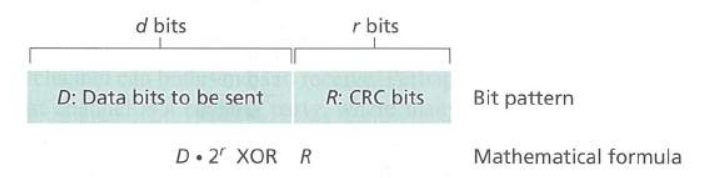
\includegraphics[width=.9\linewidth]{c:/Users/Christian/Documents/GitHub/Home/OrgFiles/Class Notes/Files/CCN Snippets/6.2.3.1.png}
\bicaption{}
\end{figure*}

\begin{figure*}
\centering
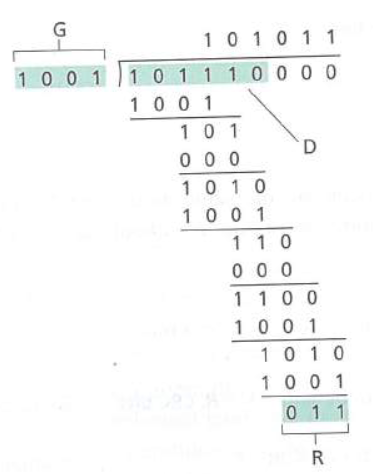
\includegraphics[width=.9\linewidth]{c:/Users/Christian/Documents/GitHub/Home/OrgFiles/Class Notes/Files/CCN Snippets/6.2.3.2.png}
\bicaption{Calculation}
\end{figure*}

\subsection{6.3 Multiple Access Links and Protocols}
\label{sec:org928990e}
Two types of network link:
\begin{itemize}
\item point to point link - single sender at one end, single receiver at the other. Many protocols designed for this; point to point protocol (PPP), high level data link protocols (HDLC) etc.
\item Broadcast link - multiple sending and receiving nodes all connected to the same shared broadcast channel. When one node transmits a frame, every other node receives a copy.

Mutiple Access Problem - how to coordinate access of multple sending and receiving nodes to a shared channel.

Multiple Access Protocol - regulates access to shared channel.

Collission - 2 packets sent/arrive at the same time. Receiving nodes cant make sense of collided nodes.

3 Categories for Multiple Access Protocols: Channel partitioning protocols, Random access protocols, Taking turns protocols.

These protocols should have the following characteristics:
\begin{enumerate}
\item When only one node is sending, that node has throughput = R bps.

\item When M nodes have data to send, each node has throughput / Average transmission rate = R/M bps.

\item Protocol decentralized, no master node /  single point of failure.

\item Protocol is simple
\end{enumerate}
\end{itemize}

\subsubsection{6.3.1 Channel Partitioning Protocols}
\label{sec:org670f710}

Recall Time and Frequency division multiplexing. Time - divides into frames and further into time slots. Frequency - divides single channel into many smaller channels with limited throughput.

Third available partitioning protocol - Code Division Multiple Access (CDMA). Assigns a code to each node. Each node uses its code to encode the data it sends. If codes are chosen carefully, different nodes can transmit simultaneously without interference. 

\subsubsection{6.3.2 Random Access Protocols}
\label{sec:org6cf352b}
In Random Access Protocols, sending node always transmits at the full rate of the channel (R bps).
When there is a collision, each node involved rapidly retransmits its frame/packet until it gets through w/o collision. Sender waits a random delay between each packet.

Lots of random examples.

\begin{enumerate}
\item Slotted ALOHA
\label{sec:orga6acaef}
\begin{itemize}
\item All frames exactly L bits
\item Time divided into L/R seconds
\item Nodes start to transmit only at the begining of slots
\item nodes are synchronized
\item if 2 or more frames collide in a slot, all nodes detect collision before slot ends

If collision, node has probability between 0 and 1 to retransmit at the beginning of the next slot. Repeats until sends successfully.
\end{itemize}

\item ALOHA
\label{sec:orgc773683}

All nodes synchronized, start transmit at beginning of slot. If node experiences collision, probability between 0 and 1 to retransmit immediately.

\item Carrier Sense Multipl Access (CSMA)
\label{sec:org2367790}
Where ALOHA retransmits repeatedly without shutting up, CSMA:
\begin{itemize}
\item Listens - \textbf{carrier sensing}; node listens to channel before sending. If frame from other node is currently being transmitted, then current node waits until channel is free
\item Stop talkink - \textbf{Collision Detection}; transmitting node listens to channel, if another node starts sending at the same time, first node stops and waits random amount of time before checking again.
\end{itemize}

\item Carrier Sense Multiple Access with Collision Detection (CSMA/CD)
\label{sec:org0ba56c4}
\begin{enumerate}
\item Adapter obtains datagram from network layer, prepares link layer frame
\item Adapter senses that channel is idle, starts to transmit or waits then starts
\item While transmitting, monitors channel for new traffic and either completes transmit, or aborts and returns to step 2.
\end{enumerate}

\item CSMA/CD Efficiency
\label{sec:org75658b3}
Efficiency = \(\frac{1}{1+5d_{prop}/d_{trans}}\)
\end{enumerate}

\subsubsection{6.3.3 Taking Turns Protocols}
\label{sec:orgdaee9b6}

2 Desirable properties of Multiple Access Protocol:
\begin{itemize}
\item When only one node active, that node has throughput of R bps.
\item When M nodes active, nodes have throughput of R/M bps

2 Types of Taking Turns Protocols

\begin{itemize}
\item Polling Protocol
Requires one of the nodes to be designated a master node. Master node \textbf{polls} each node in "round robin".
Tells Node 1 to transmit up to some maximum number of lines, then tells Node 2 the same, so on.
This creates a polling delay, but is much more reliable and produces fewer collissions than random access.

\item Token-Passing Protocol
No master node. small, special purpose frame called a \textbf{token} is exchanged among nodes in some fixed order. When a node receives a token, holds on to it only if it has some frames to transmit, else forwards. If a node has frames, it forwards up to the maximum number then forwards the token.
Extremely effective, but one node's failure can crash the entire network.
\end{itemize}
\end{itemize}

\subsubsection{6.3.4 DOCSIS: The Link-Layer Protocol for Cable}
\label{sec:orgba2b398}

Cable access network connects several thousand residential cable modems to a cable modem termination system (CMTS) at cable network headend.
Data-Over-Cable Service Interface Specifications (DOCSIS) specifies cable data network architecture and protocols.
Uses FDM to divide downstream (CMTS to modem) and upstream (Modem to CMDS) into several channels. Downstream channels 6 MHz wide, maximum throughput about 40 Mbps per channel. Upstream Channels 6.4 MHz wide, maximum throughput about 30 Mbps per channel.
Frames on the downstream channel are received by all the cable modems. Multiple cable modems share the same upstream cable modem however, makes transmitting upstream more challenging. CMTS grants explicit permission to individual modems to transmit during specific time slots. Sends control messages called a MAP message on a downstream channel to specifiy which modem can transmit during which time slots. These slots are allocated to specific modems, so helps eliminate colissions. Each modem sends request messages if they have information to send. These messages are sent during a time interval specifically dedicated for this purpose, and sent in random access manner. Resends request if no response received in certain amount of time. 

\subsection{6.4 Switched Local Area Networks}
\label{sec:org23d3c85}
\begin{figure*}
\centering
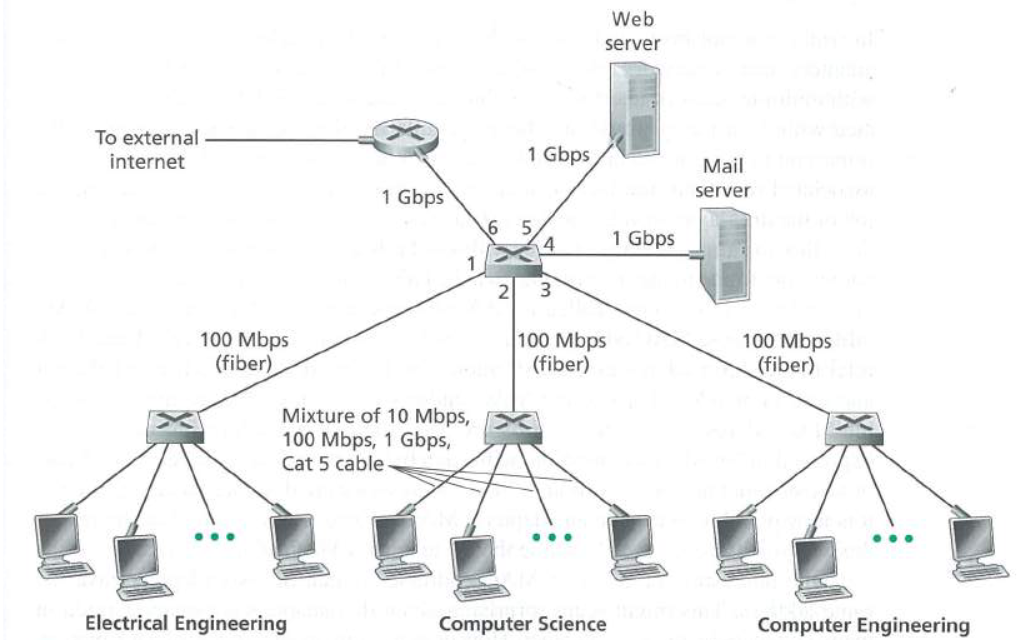
\includegraphics[width=.9\linewidth]{c:/Users/Christian/Documents/GitHub/Home/OrgFiles/Class Notes/Files/CCN Snippets/6.4.0.1.png}
\bicaption{Switched Local Area Network}
\end{figure*}

In this network, switches operate at the link layer.
They don't recognize network later addresses, use routing algorithms (like RIP or OSPF) to route paths, don't use IP addresses (use link-later addresses instead).

\subsubsection{6.4.1 Link Layer Addressing and ARP}
\label{sec:org29ba1fd}
Hosts and routers have link-layer addresses as well as network layer addresses (discussed earlier).

Address Resolution Protocol (ARP) provides mechanism to translate IP addresses to Link-Layer Addresses.

\textbf{MAC Addresses}
Not actually the hosts and routers that have link-layer addresses - it's their \emph{adapters} (network interfaces).

Link layer switches don't have link-layer addresses for connections to hosts and routers, since they only act as the connection not the interface.

Link layer address also called \uline{LAN Address}, \uline{Physical Address}, or \uline{MAC Address}.

MAC address is 6 bytes long, \(2^{48}\) possible addresses. Typically in Hexadecimal notation.
Addresses are constant (can technically be changed, but were designed to be permanent).
Every adapter has a different Address - managed by IEEE (almost like an SSN, while an IP address is like a mailing address).

\textbf{Address Resolution Protocol} (ARP)

ARP translates between network layer addresses (like IP) and link layer addresses.
\begin{figure*}
\centering
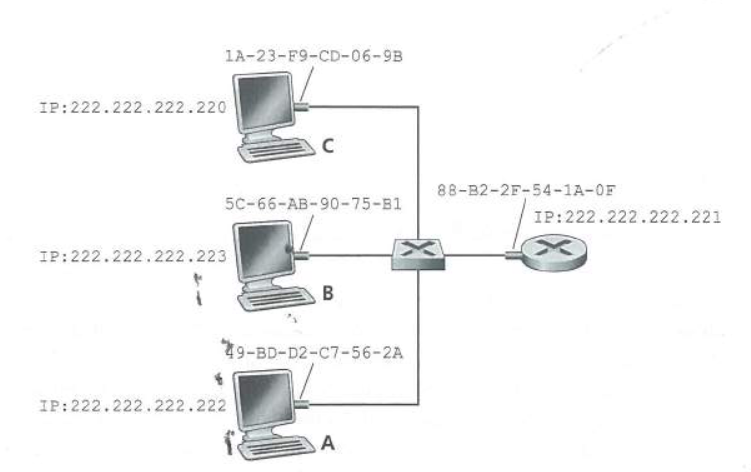
\includegraphics[width=.9\linewidth]{c:/Users/Christian/Documents/GitHub/Home/OrgFiles/Class Notes/Files/CCN Snippets/6.4.1.1.png}
\bicaption{Network Layer and Link Layer Addresses}
\end{figure*}

When forwarding a packet, source must give its adapter the correct destination IP address and MAC address. Uses ARP to match IP addresses to MAC addresses. Uses ARP tables (just like every other routing protocol we've looked at). If there's no preexisting entry, ARP constructs an \emph{ARP packet}. Has several fields - sending/receiving IP and MAC addresses. Query and response messages have same format. Simply queries every other host on the network to determine IP addresses and the corresponding MAC address. ARP query is sent in a broadcast frame, response is sent in a standard frame. ARP tables get configured automatically. If host is disconnected, its entry is deleted.

ARP protocol is a special case - both link layer and network layer - straddles boundary.

\textbf{Sending a Datagram off the Subnet}
\begin{figure*}
\centering
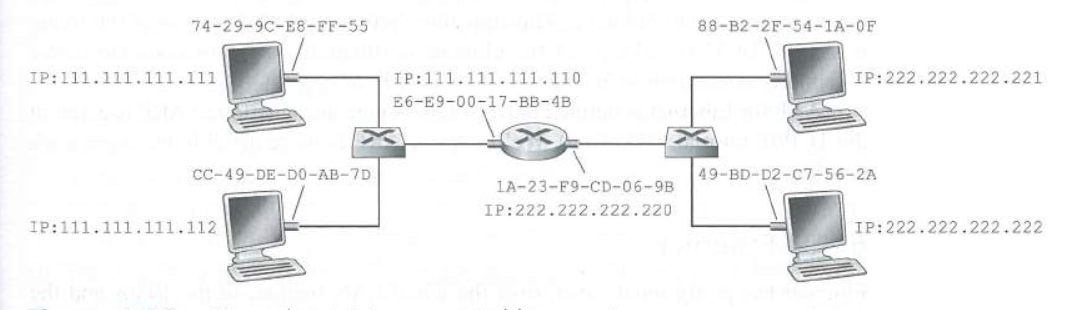
\includegraphics[width=.9\linewidth]{c:/Users/Christian/Documents/GitHub/Home/OrgFiles/Class Notes/Files/CCN Snippets/6.4.1.2.png}
\bicaption{Two Subnets Connected by a Router}
\end{figure*}

In this diagram, the router in the center is connected to two subnets. Therefore has 2 interfaces, and 2 MAC/IP addresses.

Would be reasonable to assume that the destination MAC address would be that of the destination host on the other network. WRONG. Since that MAC address isn't in this subnet, the packet would not get routed.

Instead, we use the MAC address for the interface that bridges the two networks, sending a \emph{Frame} containing the true datagram to this interface. The datagram is seperated from the frame in the router and encapsulted into a new one, so that now the destination MAC address matches the true destination. Done via an ARP package. 

\subsubsection{6.4.2 Ethernet}
\label{sec:orgc4c5a54}

Ethernet - first widely deployed high speed LAN. Other methods were more expensive and complicated.

Original Ethernet developed mid-1970's (Bob Metcalfe and David Boggs).
Used a coax bus to connect nodes.
Bus topology lasted to mid-80's. Using this topology, Ethernet was a broadcast LAN.

Hub-based star topology replaced this. Hosts and routers connected to central hib via twisted-pair copper wires. \textbf{Hub} - physical layer device. acts on individual bits instead of frames. Acts as connecter and repeater. (still broadcast).

Early 2000's - hub replaced with a switch. Switches are collissionless, but are also store and forward packet switches.

\begin{figure*}
\centering
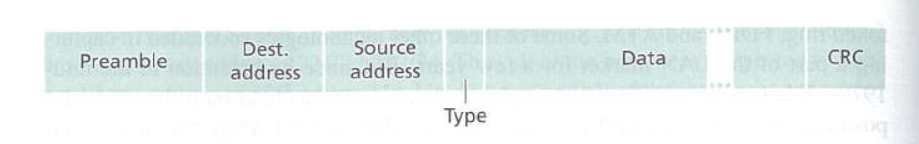
\includegraphics[width=.9\linewidth]{c:/Users/Christian/Documents/GitHub/Home/OrgFiles/Class Notes/Files/CCN Snippets/6.4.2.1.png}
\bicaption{Ethernet Frame Structure}
\end{figure*}

\begin{itemize}
\item Data Field (46-1500 bytes) -  Carries IP datagram. If higher than 1500 bytes, must fragment.
\item Destination Address (6 bytes) - MAC address of receiver
\item Source Address (6 bytes) - MAC address of sender.
\item Type Field (2 bytes) - Allows ethernet to multiplex network layer protocols.
\item Cyclic-Recundancy Check (4 bytes) - Allows receiving adapter to detect errors in the frame.
\item Preamble (8 bytes) - First 7 bites are "10101010" last byte is "10101011". Serves to "wake up" the receiving adapters and synchronize their clocks to the senders clock.

Ethernet has been standardized at 100 Mbps.

Gigabit Ethernet:
\begin{itemize}
\item Uses standard ethernet frame format, backwards compatible

\item Allows for point to point links and shared broadcast channels.

\item Uses CSMA/CD for shared broadcast channels.

\item Allows for full duplex operation (40 Gbps in both directions for Point to Point).
\end{itemize}
\end{itemize}

\subsubsection{6.4.3 Link-Layer Switches}
\label{sec:org7b4e819}
Switches - forward link-layer frames to outgoing links.
Switch it \emph{transparent} to hosts and routers in the same subnet - means that nothing actually addresses to the switch itself, switch is a passthrough point in a route to another host/server.

Switches have buffers.

\textbf{Forwarding and Filtering}
Filtering - process to determine whether a frame ought to be forwarded or dropped.
Forwarding - switch function. Determines which interfaces a frame should go to, then transports frame to those interfaces.

Processes done with a switch table.

Switches can be used to forward with MAC addresses.

How filtering and forwarding work:
Given destination address DD-DD-DD-DD-DD-DD

Frame arrives at switch for interface \emph{x}.
Switch indexes to table for MAC address DD-DD-DD-DD-DD-DD.

3 cases:
\begin{itemize}
\item No entry for destination address. Switch broadcasts the frame.
\item An entry exists, for DD-DD-DD-DD-DD-DD in interface \emph{x}. I.E. Local origin, local destination. Switch doesn't need to forward, since the destination is local. Switch can drop the frame since other routing methods handle local forwarding.
\item An entry exists, for DD-DD-DD-DD-DD-DD in interface \emph{y} (not \emph{x}). Frame must be forwarded outside the LAN. The switch forwards the frame to the interface that's connected to \emph{y}.
\end{itemize}


\textbf{Self-Learning}
Tables are built automatically (self learning).
\begin{enumerate}
\item Table starts out empty
\item Whenever an incoming frame arrives at an interface, switch stores MAC address, Source Address Field, Source Interface, Current Time.
\item Switch deletes addresses from which it doesn't receive any frames after a set variable (\textbf{aging time}).

\textbf{Properties of Link Layer Switching}
\begin{itemize}
\item \emph{Elimination of Collisions} - LANs made from switches, no collisions. Switches use their buffers to transmit only one frame at a time.

\item \emph{Heterogenous Links} - Switches isolate links from each other, so different links can run at different speeds. Helps to combine older equipment with new/faster components.

\item \emph{Management} - Switches can detect potential malfunctions, and disconnect from the offending router. Cut cables only disconnect the host that was connected to that cable. Previously, coax lines were like those crappy christmas lights. One goes out they all go out.
\end{itemize}
\end{enumerate}


\textbf{Switches vs Routers}
Routers - store and forward packet switches, use network layer addresses. Layer 3. Packets not restricted - can use "best possible path". Have firewalls - protect against high traffic/overload. Not plug and play. More processing delay. 


Switches - store and forward packet switches, use MAC addresses. Layer 2. Plug and Play. Higher filtering/forwarding rates. More restricted topology. Higher traffic/overload possible.

Switches better for smaller networks. Routers "isolate traffic" better, handle larger volumes more effectively. 

\subsubsection{6.4.4 Virtual Local Area Networks (VLANs)}
\label{sec:org8e93333}
Most modern LANs - based on a hierarchy
\begin{itemize}
\item Switched LANs in layers to form a tiered structure
\end{itemize}


Drawbacks to this architecture:
\begin{itemize}
\item \emph{Lack of Traffic Isolation} - Even though most messages have a dedicated path, and have optimized routes, traffic that doesn't have a destination (like ARK and DHCP messages, whose destination is computed later) have to broadcast to the entire network in order to collect the information they need.
\item \emph{Inefficient Use of Switches} - Depending on the size of the network, we can trade several tiered switches for one single switch (still has drawbacks)
\item \emph{Managing Users} - Hosts are connected via physical cables. If a host moves, so too must the phyisical cable connections.
\end{itemize}


These issues are solved by VLANs.
They create a "virtual" local area network on a single physical switch. Inside each VLAN, hosts can connect as if they were on an isolated network.
Since they're isolated, how can we talk between VLANs?
We can effectively connect two ports on each VLAN as if they were connected via a router. Then functions like a normal, 2 network system.

Better method is called \textbf{VLAN Trunking}.
Uses "Trunk Ports" to connect two VLAN switches. This port is a part of each VLAN. In order to properly route between several VLANs, uses a 4 bit \textbf{VLAN Tag} to identify the source VLAN.
Tag is 2 bytes of Tag Protocol Identifier (TPID) and 2 bytes of Tag Control Information
12-bit VLAN Identifier Field, 3-bit Priority Field. 

\subsection{6.5 Link Virtualization: A Network as a Link Layer}
\label{sec:org1be15f6}

Link: previously seen them as physical connections, more ephemeral "bands" or "channels", and in wider senses.

\subsubsection{6.5.1 MultiProtocol Label Switching (MPLS)}
\label{sec:org37d9be7}

Merges IP forwarding system with "labels". Selectively labels datagrams and lets routers forward based on these labels (This is in place of IP addresses when possible).

MPLS header contains Label, Exp Field, S and TTL

EXP - 3 bits for experiments.
S - Notes the end of "stacked" MPLS headers.
TTL - time to live

MPLS is not compatible with non-MPLS routers. MPLS capable - known as "\textbf{Label-Switched}"


\begin{figure*}
\centering
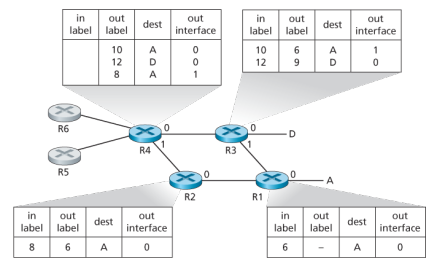
\includegraphics[width=.9\linewidth]{/home/chris7701/Github/Home/OrgFiles/Class Notes/Files/CCN Snippets/6.5.1.1.png}
\bicaption{MPLS Basic Structure}
\end{figure*}

R1 through R4 are MPLS compatible. R5 and 6 are IP, non MPLS.
R1 communicates to R2 and 3 that it can send to Destination A. R3 communicates to R4 that it can send to A and D, and that it will send frames with label 10 and label 12 to each of those locations respectively. R2 communicates to R4 that it can send to A. R4 has two options to reach A.

MPLS helps increase switching speeds, but also allows new ways to manage traffic. MPLS opens up more route options which can help reduce congestion on other paths. Also used to implement \textbf{Virtual Private Networks} (VPN's). 

\subsection{6.6 Data Center Networking}
\label{sec:orgb991504}

Large companies use data centers to store transmit and route information. Data centers have their own \textbf{Data Center Networks}.
Hosts (\textbf{blades}) are arranged in server racks. Each has about 40 blades. Each rack has a switch, called the \textbf{Top of Rack Switch} (TOR).
Each rack's NIC connects to this switch. Ports allow routing between switches.

Data Center Network allows internal and external traffic.

\begin{figure*}
\centering
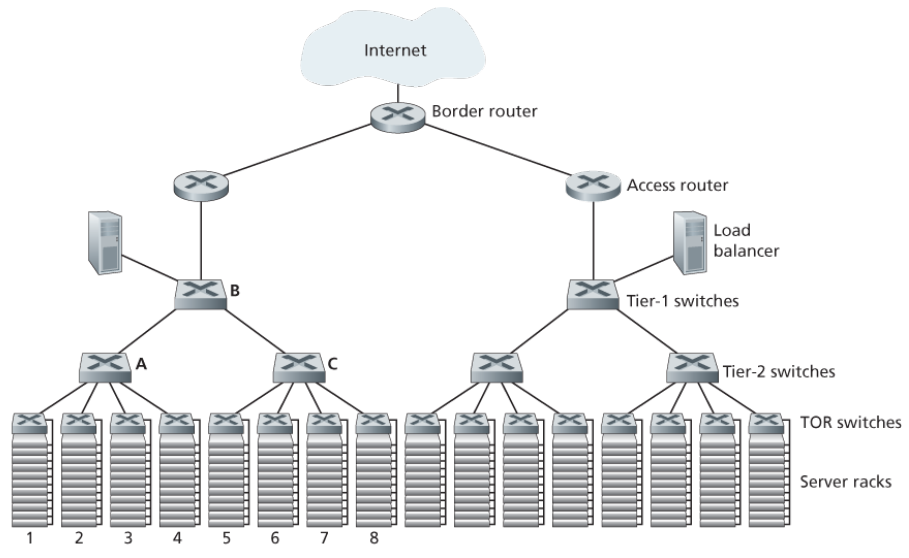
\includegraphics[width=.9\linewidth]{/home/chris7701/Github/Home/OrgFiles/Class Notes/Files/CCN Snippets/6.6.0.1.png}
\bicaption{Data Center Network - Hierarchical Topology}
\end{figure*}

\textbf{Load Balancing}

Incoming requests are sent to a \textbf{load balancer} before they are router to servers or applications inside the data center. Load Balancer distributes requests among the different hosts, reducing overall strain. Also called "layer 4 switches". Can serve as a sort of NAT, allowing communication between external and internal networks.

\textbf{Hierarchical Architecture}

Small Data Center - border router, load balancer, about 30 racks (likely connected by a single physical ethernet switch).

Scaling up - hierarchy made up of routers and switches.
Border Router accesses external networks.
Each access router has 3 tiers below it, top level is a "top-tier switch", these connect to several second-tier switches, and these connect to even more third tier switches (which are actually the TOR switches, leading to racks of hosts).

This allows connection to external networks, but connection between large number of internal hosts is still somewhat troublesome. While everything is connected, the max speed each host is allowed on a local level is relatively slow. 

\subsection{6.7 Retrospective: A Day in the Life of a Web Page Request}
\label{sec:org9ea045a}

\subsubsection{6.7.1 Getting started: DHCP, UDP, IP, and Ethernet}
\label{sec:org813db22}

Computer connected via Ethernet cable and switch to Router.
Router connected to ISP.
ISP provides DNS access to the router (and thereby to each host).


\begin{figure*}
\centering
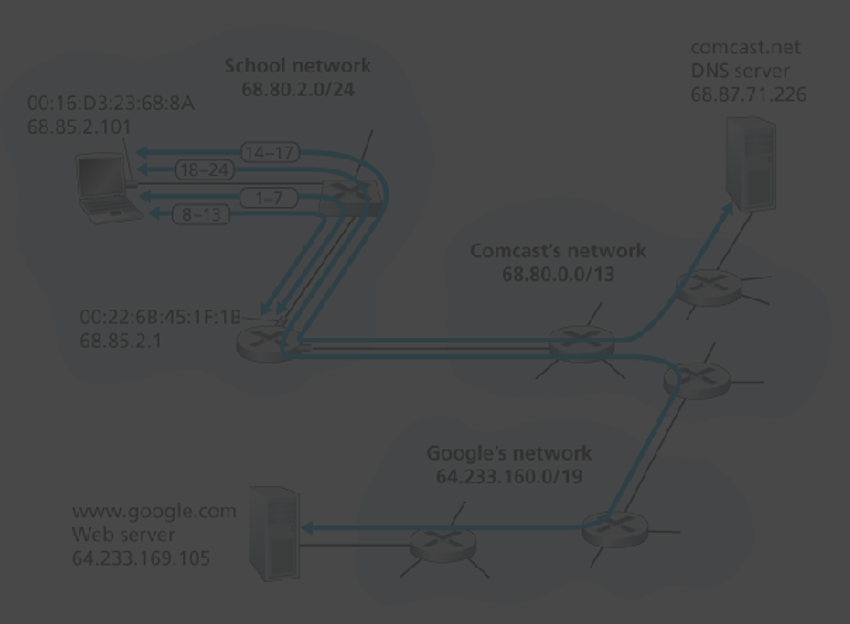
\includegraphics[width=.9\linewidth]{/home/chris7701/Github/Home/OrgFiles/Class Notes/Files/CCN Snippets/6.7.1.1.png}
\bicaption{Scenario Overview}
\end{figure*}

Bob obtains an IP address from DHCP (This is automatic).

Steps:

\begin{enumerate}
\item Computer creates a \textbf{DHCP Message Request}. Encapsulates this inside a UDP Segment (destination port 67 - to the DHCP server and source port 68). Then places the UDP segment inside an IP datagram, and broadcasts it.
\item IP datagram goes inside an Ethernet frame with a Destination MAC address - FF:FF:FF:FF:FF:FF. This is basically just the link-layer version of an IP broadcast.
\item Since this is the first frame the DHCP switch will receive from the host, entries will be made in all router/etc along the way.
\item Router receives the Ethernet frame, pulls out the IP datagram, and sends that up. The package is demultiplexed all the way to the DHCP server, where it extracts the initial \textbf{DHCP Message Request} and processes it.
\item DHCP server creates ACK message with the IP address it wants to assign to the host. ACK also contains the IP of the DNS server, the default gateway, and the network mask (subnet). Puts this in the same level of encapsulation as the incoming message had (UDP segment inside IP datagram inside Ethernet frame).
\item Packet is sent. essentially follows the same route as the original back to the Host computer. Switch is able to properly route the package because it is \textbf{self-learning} and remembered the destination from the original packet it received from the host.
\item Once the host receives the package, it extracts each successive encapsulation. Records the IP addresses contained in the ACK message.
\end{enumerate}

\subsubsection{6.7.2 Still Getting Started: DNS and ARP}
\label{sec:org3c98219}

Whenever a host tries to access the internet, it creates a \textbf{TCP Socket} in order to send an \textbf{HTTPS Request} to the website.

\begin{enumerate}
\item Host OS creates \textbf{DNS query message} to find the website it wants. Sends to the DNS server, but doesn't know the MAC address for the gateway. (knows Ip from DNS, not mac)
\item Uses ARP to find MAC Address.
\item \textbf{ARP Query} - target IP as the default gateway. Broadcasts this over link layer (FF:FF:FF:FF:FF:FF). Router receives, sends out to everybody.
\item Gateway receives, recognizes its own IP in the ARP Request, responds - \textbf{ARP Reply} - contains own MAC address, etc.
\item Host receives, extracts information.
\item Host is now able to address the real DNS query to the default gateway. Frame destination address (Link Layer) is the default gateway. IP destination is the DNS server.
\end{enumerate}

\subsubsection{6.7.3 Still Getting Started: Intra-Domain Routing to the DNS Server}
\label{sec:orgf744714}

\begin{enumerate}
\item Gateway receives, extracts IP for DNS query. FIgures out which router to direct it to.
\item Destination router receives, extracts IP datagram, and uses the routing table to find the appropriate interface to send it to. This depends on the necessary protocol (RIP, OSPF, or IS-IS.
\item DNS Query gets to the DNS server. Server looks up the website. Extracts the IP address (cached in the Authoritative Server). Sends \textbf{DNS Reply} back, encapsulated in UDP segment and IP datagram.
\item Host extracts the IP, now it has the destination to send the initial request from the very beginning. (i.e. bob wanted to send a letter, now he has the address to send it to.)
\end{enumerate}

\subsubsection{6.7.4 Web Client-Server Interaction: TCP and HTTP}
\label{sec:orgad30bc5}
\begin{enumerate}
\item Host creates \textbf{TCP Socket} it will use for the HTTP GET message. Host uses TCP for \textbf{Three Way Handshake} with google.com (destination website). Host then creates TCP SYN segment (HTTP uses port 80) and creates TCP segment in IP datagram with destination IP of 64.233.169.105, then puts this in a link-layer frame addressed to the Gateway's MAC address.
\item Datagram is forwarded to destination website.
\item Datagram with TCP SYN gets to destination site. Message is extracted, demultiplexed to port 80. Connection socket created. TCP SYNACK - segment generated (message inside datagram inside link layer)
\item Forwarded through Website to Host. Demultiplexed to TCP socket created in the host earlier.
\item Socket is now ready to send information to website. Browser creates HTTP GET message, sends to Hosts socket, GET message becomes payload of TCP segment inside a datagram and send to Website.
\item HTTP server at website receives, creates HTTP Response, sends HTTP Response back through its TCP socket. Host receives; displays page.
\end{enumerate}

\section{Chapter 7 - Wireless and Mobile Networks}
\label{sec:org72ef512}

\subsection{7.1 Introduction}
\label{sec:orgec89cfd}
Parts of a wireless network
\begin{itemize}
\item Wireless Hosts
Anything that runs applications. Laptop, Phone, etc.
\item Wireless Links
Wireless Communication Links are the conduits through which hosts connect to wireless procviders (base stations).
2 important characteristics - coverage area and link rate
This is basically what provides the "wireless" component to the network, at least on a local/small scale.
\item Base Station
Theres no real parallel to this in a wired network. This is what gives wireless connection on a larger scale. Think cell towers or wifi hotspots.
When hosts are connected to a base station - called operating in "Infrastructure Mode"
Ad Hoc networks - wireless hosts don't have this infrastructure provided by the base station
\item Network Infrastructure
The larger, external network the host communicates with
\end{itemize}


Different types of Wireless Networks (differentiated by \emph{One hop vs Multiple} and whether there is \emph{Infrastructure})
\begin{itemize}
\item Single Hop, Infrastructure Based
Base station is connected to larger network. All communication between station and host spans a single hop. Most networks.
\item Single Hop, Infrastructure-less
No base station. One of the nodes may act as the central point. Bluetooth uses this structure.
\item Multi-Hop, Infrastructure Based
Base station is present, but some nodes may be seperated from the station. They need to connect to other nodes in order to access the base station. Wireless sensor networks and Wireless Mesh Networks.
\item Multi-Hop Infrastructure-less
No base station, nodes rely on other nodes. Some may be mobile. Mobile Ad Hoc Networks (MANET) and Vehicular Ad Hoc Networks (VANET).
\end{itemize}

\subsection{7.2 Wireless Links and Network Characteristics}
\label{sec:org8a5c788}
Differences between a wired and wireless link
\begin{itemize}
\item Signal Strength
Wireless signals decrease in strength over distance (known as path loss)
\item Interference from other sources
When multiple radio sources are transmitting at the same frequency, they interfere with each other (think constructive/destructive interference from Physics. Both are bad.)

\item Multipath Propogation
When some portions reflect off hard surfaces and others dont. Can cause distortion (pieces of the signal arrive "out of order" etc)
\end{itemize}


Signal to Noise Ratio - Relative measure of strength. Measured in dB.

Given Modulation scheme - SNR and BER inversely proportional
Given SNR - bit transmission rate proportional to BER
Dynamic Selection for Physical Layer Modulation - helps adapt the modulation technique to channel conditions

\subsubsection{7.2.1 CDMA}
\label{sec:org2c8b10e}
CDMA encodes bits by multiplying them  by a signal/"code" that constantly changes.
Theres a bunch of math involved.
\(Z_{i,m} = d_{i} * c_{m}\)(basically just number times code).
Recover the word with \(d_{i} = \frac{1}{M}\sum\limits_{m=1}^{M}{Z_{i,m}*c{m}}\)
With multiple senders, there's interference, so computation changes.
\(Z_{i,m}^{*} = \sum\limits_{s=1}^{N}{Z_{i,m}^{s}}\)
Each sender can (magically? idk, math\ldots{}) pull the recovered data using
\(d_{i} = \frac{1}{M}\sum\limits_{m=1}^{M}{Z_{i,m}^{*}*c_{m}}\)



\section{Chapter 8 - Security in Computer Networks}
\label{sec:orgbc742df}

\subsection{8.8 - Securing Wireless LANs}
\label{sec:org42496fa}
Wired Equivalent Privacy - the collective, standardized security mechanisms in place over the internet.

\subsubsection{8.8.1 Wired Equivalent Privacy}
\label{sec:org33381a4}
provides authentication. Encrypts data between a host and wireless access point . Uses a "symmetric shared key", but doesn't manage the key itself, instead assuming that the host and wireless access point have agreed on a key ahead of time.

Steps:
\begin{enumerate}
\item Wireless host requests authentication through an access point
\item Access point responds to the request with a 128-byte "nonce value"
\item Wireless host encrypts the nonce with the key
\item Access point decrypts the nonce after its encrypted by the nonce
\end{enumerate}


If the newly decrypted nonce matches the original sent value then the access point considers the host "authenticated".
Steps for encryption:
4-bit CRC value generated for the data. Payload and CRC bytes are encrypted with the RC4 cipher, which produces key values which the system uses to encrypt the data and CRC bytes. Bits of ciphertext are made by XORing ith bit of data with ith key.
\(c_{i} = d_{i} \oplus k_{i}^{IV}\)
IV value changes with each frame. Included (in plaintext) in each encrypted headers frame. Receiver takes its key appends the IV and uses the result to decrypt.
\(d_{i} = c_{i} \oplus k_{i}^{IV}\) and we also have \(d_{i} \oplus c_{i} = k_{i}^{IV}\)

\subsubsection{8.8.2 IEEE 802.11i}
\label{sec:org6571e07}
Replaces 802.11. Stronger security mechanisms. Seperates the authentication server from the AP.
Four phases:
\begin{enumerate}
\item Discovery
AP advertises its presecence, forms of authentication/encryption. Client requests specific types of authentication/encryption that it wants. Client isn't yet authenticated, doesn't have encryption key.
\item Mutual authentication and Master Key generation
Authentication takes place (client and server). Access point is a relay, forwarding between client and server. "Extensible Authentication Protocol (EAP)" announces the end-to-end format the messages take. These messages are encapsulated with EAPol (EAP over LAN). Then decapsulated at the access point and encapsulated again with the RADIUS protocol in order to transmit over UDP/IP. This part isn't required, but its pretty much the standard. DIAMETER is likely to replace RADIUS.
\item Pairwise Master Key generation
Master key is a shared secret which only the client and the auth server know. They each use this to make a "pairwise master key"which they send to the AP.
\item Temporal Key Generation
PMK allows the Client and AP to generate more keys to help with communication. They use the temporal key to do link-level encryption.
\end{enumerate}



\subsection{8.9 Operational Security: Firewalls and Intrusion Detection Systems}
\label{sec:orgb22a5c0}

\subsubsection{8.9.1 Firewalls}
\label{sec:orgecf0ad2}
firewall - combination of hardware and software. Seperates an internal network and its contents from the external internet. Regulates traffic through the divide.

3 goals:
\begin{itemize}
\item Ensure that all traffic in both directions passes through the firewall
\item Only authorized traffic is allowed to pass
\item Firewall itself is immune to penetration
\end{itemize}


Two leading vendors - Cisco and CheckPoint
Three categories of firewalls: traditional packet filters, stateful filters, application gateways

\textbf{Packet Filters}
Traffic always passes through a router to enter or leave a network.
Filtering decisions are made based on IP source/destination, Protocol Type, TCP/UDP source/destination port, TCP flags  (SYN, ACK, etc), ICMP Message Type, Different rules for datagrams entering the network, Different rules for different router interfaces.

\textbf{Stateful}
Filter based on TCP connections
Observes a three way handshake to take information from packet headers. 

\textbf{Application Gateway}
Firewalls are specific to applications. Each is a seperately running server through which all packets must pass.
If users have permission, then the gateway:
\begin{itemize}
\item prompts for the external host to which it wants to connect
\item Creates a gateway session between gateway and host
\item Relays all the data arriving from the user to the external destination
\end{itemize}


\subsubsection{8.9.2 Intrusion Detection Systems}
\label{sec:org2bfac26}
Intrusion Detection System - looks for malicious traffic and alerts if it finds any.
Intrusion Prevention System - actually blocks the traffic once it detects it

IDS - either signature or anomaly based.
signature based - keeps a database of attack signatures
Anomaly based - creates a traffic profile based on normal operation


\textbf{Snort}
open source IDS.
\end{document}